%Latex document for ESSDERC 2021 Paper 

\documentclass[10pt,a4paper,twocolumn]{article}
\usepackage[utf8]{inputenc}
\usepackage{authblk}
\usepackage{amsmath}
\usepackage{nccmath} % added this
\usepackage{amsfonts}
\usepackage{amssymb}
\usepackage{makeidx}
\usepackage{graphicx}
\usepackage{fourier}
\usepackage[ruled,vlined]{algorithm2e}
\usepackage{empheq}

\setlength{\parindent}{0pt}
\usepackage[left=1cm,right=1cm,top=1cm,bottom=2cm]{geometry}

% Title
\title{3D Simulation of PDE and Jitter in SPAD Devices.}

% AUthors and affiliation
\author[1]{Rémi Helleboid}
\author[1]{Denis Rideau}
\author[2]{Norbert Moussy}
\author[2]{Olivier Saxod}
\author[1]{Jeremy Grebot}
\author[1]{Isobel Nicholson}
\author[1]{Antonin Zimmerman}
\author[1]{Sara Pellegrini}

\affil[1]{ST Microelectronics, Crolles, France}
\affil[2]{CEA LETI, Grenoble, France}

\date{}                     %% To hide the date
\setcounter{Maxaffil}{0}
\renewcommand\Affilfont{\itshape\small}
% Keywords command
\providecommand{\keywords}[1]
{
  \small	
  \textbf{\textit{Keywords---}} #1
}


\begin{document}


% Title
\maketitle

% Abstract
\begin{abstract}
In this paper we present a full 3D simulation methodology to extract Photon Detection Probability (PDP) and Jitter of Single-Photon Avalanche Diode (SPAD) Devices. The simulation results are compared with measurements on devices and show good agreement with the experiments.\\
\end{abstract}

% Keywords
\keywords{single-photon avalanche diode (SPAD), photon detection probability (PDP), jitter, avalanche breakdown probability, breakdown voltage}

% Introduction
\section{Introduction}
Single Photon Avalanche Diodes (SPAD) are key optoelectronic detectors for medical imaging, camera ranging and automotive laser imaging detection and ranging (LiDAR) applications. Currently, the device leading the market is a micrometric silicon (Si) PN junction associated to a proximity CMOS electronics biasing the system above the breakdown voltage. Si-SPADs present low noise and relatively high photon detection probability (PDP), but their sensitivity is limited to photon wavelengths lower than 1100 nm, while class 1 eye-safety devices would require wavelengths larger than 1400 nm.


\section{Device structure and TCAD simulation}
\begin{figure}[hbtp]
\caption{SPAD simulation workflow}
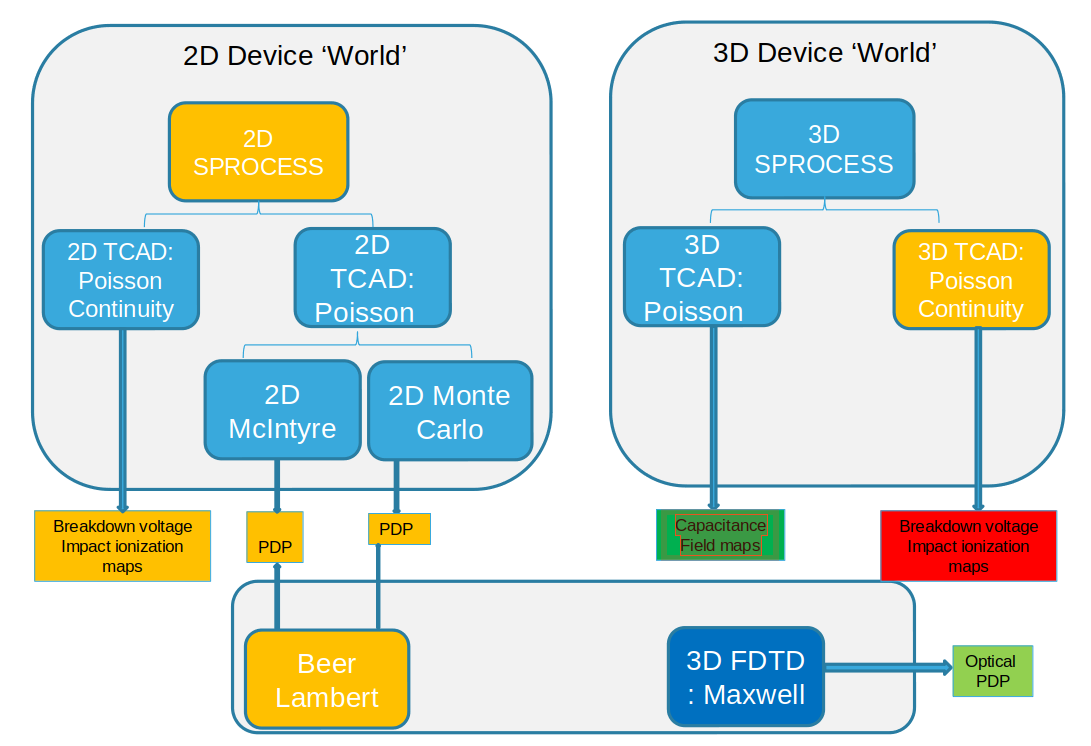
\includegraphics[scale=0.21]{../pictures/TCADWorkflow.png}
\end{figure}


\section{Avalanche breakdown probability}
The avalanche breakdown probability is computed by the means of the well known McIntyre model \cite{oldham_triggering_1972}. We briefly recall the model derivation : 
Let $P_e(x)$ be the probability that an electron starting at x in the depletion layer triggers an avalanche and $P_h(x)$ the same probability for an hole starting at x.
Straightforwardly, the probability that neither an hole nor an electron starting at x trigger an avalanche is given by $(1-P_e(x))(1-P_h(x))$.
Thus, the probability that either the hole or the electron trigger an avalanche, noted $P_{pair}$ is :
\begin{align*}
P_{pair}(x) &= 1 - \left( 1-P_e(x)\right)\left(1-P_h(x)\right)  \\
			&= P_e + P_h - P_e P_h
\end{align*}

Now, the probability that an electron starting at $x+dx$ triggers an avalanche is :
The probability that the electron reaches the position $x$ and triggers an avalanche in $x$ plus the probability that it triggers an avalanche between $x$ and $x+dx$ less the probability of the intersection of the two previous events. It writes : 
\begin{align*}
P_e(x+dx) &= P_e(x) + \alpha_e(x) dx P_{pair}(x)  - P_e(x)  \alpha_e dx P_{pair}(x) \\
		  &= P_e(x) + \alpha_e(x) dx (P_e(x) + P_h(x) - P_e(x) P_h(x)) \\& \qquad - P_e(x) \alpha_e(x) dx (P_e(x) + P_h(x) - P_e(x) P_h(x)) \\
		  &=  P_e(x) + dx \, \alpha_e(x) (P_e(x) + P_h(x) - P_e(x) P_h(x)) (1 - P_e(x))
\end{align*}
Where $\alpha_e$ is the electron linear ionization rate : the probability by length that an electron create an impact ionization event.  \\
One can rearrange the terms to obtain : 
\[ \frac{P_e(x+dx)-P_e(x)}{dx} = \alpha_e(x) (P_e(x) + P_h(x) - P_e(x) P_h(x)) (1 - P_e(x)) \]
Which leads to the first ordinary differential equation : 
\[ \frac{dP_e}{dx} = (1-P_e)\alpha_e(P_e + P_h - P_e  P_h) \]

The same reasoning applies to the probability that an hole starting at $x-dx$ triggers an avalanche.
Which leads to the second ordinary differential equation : 
\[ \frac{dP_h}{dx} = -(1-P_h)\alpha_h(P_e + P_h - P_e  P_h) \]

Therefore we can draw up the McIntyre system : 

\begin{empheq}[left=\empheqlbrace]{align}
&\frac{dP_e}{dx} = (1-P_e)\alpha_e(P_e + P_h - P_e  P_h) \\
&\frac{dP_h}{dx} = -(1-P_h)\alpha_h(P_e + P_h - P_e  P_h) 
\end{empheq}
for $ 0 \leq x \leq W$. \\
Adding the couple of boundary value conditions
 : 
\begin{empheq}[left=\empheqlbrace]{align}
& P_e(x=0) = 0 \\
& P_h(x=W) = 0 
\end{empheq}
we have a full 1D coupled and non-linear boundary value problem.
Since we have to extract this value at a large number of points, we use a self-made solver, embedded in a C++ program. This solver uses finite difference method coupled with a Newton's method to care of the non-linearity of the problem \cite{ascher_numerical_1987}. The algorithm is different from those implemented in MatLab routine $\textrm{(bvp4c)}$ or SciPy function $\textrm{(solve\_bvp)}$ \cite{kierzenka_bvp_2001} but the comparison with these tools show no difference. \\
We set the following notations : 
 \[ Y(x) = \begin{pmatrix}
P_e(x) \\
P_h(x)
\end{pmatrix}
 \]

 \[ f(Y, x) = \begin{pmatrix}
(1-Y_1(x))\alpha_e(Y_1(x) + Y_2(x) - Y_1(x)  Y_2(x)) \\
-(1-Y_2(x))\alpha_h(Y_1(x) + Y_2(x) - Y_1(x)  Y_2(x)) 
\end{pmatrix}
\]

\[ g(s_1, s_2) = \begin{pmatrix}
s_1 \\
s_2
\end{pmatrix} \]

The problem hence reads : 
\begin{empheq}[left=\empheqlbrace]{align}\label{BVP_Prob}
	&Y'(x) = f(Y, x) \\
	&g(Y(0), Y(w)) = 0
\end{empheq}


\subsection{Newton scheme}
\subsubsection{Finite differences approximation}
Let $\mathcal{M}$ be the mesh on which we work. It is given by the streamlines construction. So we have : 
\[\mathcal{M}: 0 = x_1 < x_2 < x_3 < \cdots < x_N < x_{N+1} = w \]
The approximated solution on mesh $\mathcal{M}$ is $Y_{\mathcal{M}} = (y_1, y_2, \cdots, y_N, y_{N+1})$, where $y_i$ is the approximation of $Y(x_i)$.\\
For numerical approximation we again consider the mesh $\mathcal{M}$ and denote the vector of approximate solution values at mesh points by $Y_{\mathcal{M}}$. The trapezoidal scheme of finite difference methods is given by : 
\begin{align}\label{TrapezScheme}
&\frac{y_{i+1}-y_{i}}{h_{i}}=\frac{1}{2}\left(f\left(x_{i+1}, y_{i+1}\right)+f\left(x_{i}, y_{i}\right)\right) \quad 1 \leq i \leq N \\
&\quad g\left(y_{1}, y_{N+1}\right)=0
\end{align}
Thus we obtain a system of $2(N +1)$ algebraic equations for the $2(N +1)$ unknowns $Y_{\mathcal{M}}$. Unlike before, though, these equations are non-linear. The number $N$ depends on the precision we take when we construct the streamlines. We commonly take a range of $\left[1nm, 10nm\right]$, we then have $N \sim 5000$. \\
Fortunately, the Jacobian matrix of this system is rather sparse, as we shall see below.

\subsubsection{Newton method}
We consider a system of equation written in the compact form : \[ \textbf{F(s) = 0} \]
We define a function \textbf{G} : 
\[  \textbf{G}(\textbf{s}) = \textbf{s} - \left[\textbf{F}'(\textbf{s}) \right]^{-1} \textbf{F}(\textbf{s})\]
with $\textbf{F}'(\textbf{s})^{-1} $ the inverse of the Jacobian matrix of F : 
\[\textbf{F}'(\textbf{s}) = \frac{\partial\textbf{F}(\textbf{s}) }{\partial \textbf{s}}  \]

Then the newton method iterative method is given by the iteration : 
\[\textbf{s}^{k+1} =  \textbf{G}(\textbf{s}^k) \]

So the algorithm will first solve the linear system : 
\begin{equation}
\mathbf{F}^{\prime}\left(\mathbf{s}^{k}\right) \boldsymbol{\xi}=-\mathbf{F}\left(\mathbf{s}^{k}\right)
\end{equation} 
And then simply do : 
\begin{equation}
\textbf{s}^{k+1} = \textbf{s}^{k} + \boldsymbol{\xi}
\end{equation} 

\subsubsection{Construction of the linear system}

Let $\textbf{N}_{\mathcal{M}}$ be the following discrete differential operator : 
\[ \textbf{N}_{\mathcal{M}} \textbf{y}_i = \frac{y_{i+1}-y_{i}}{h_{i}}-\frac{1}{2}\left(f\left(x_{i+1}, y_{i+1}\right)+f\left(x_{i}, y_{i}\right)\right) \]

Then \[ \textbf{F}(\textbf{s}) = \begin{pmatrix}
N_{\mathcal{M}}\textbf{y}_1 \\
N_{\mathcal{M}}\textbf{y}_1 \\
\vdots \\
N_{\mathcal{M}}\textbf{y}_N \\
g(y_1, y_{N+1})
\end{pmatrix}
 \] 
We set
\[  \boldsymbol{\xi} = \begin{pmatrix}
\textbf{w}_1 \\
\textbf{w}_2 \\
\vdots \\
\textbf{w}_N \\
\textbf{w}_{N+1}
\end{pmatrix}
\]
So that the Newton method iteration becomes : 
\begin{equation}
\frac{\mathbf{w}_{i+1}-\mathbf{w}_{i}}{h_{i}}-\frac{1}{2}\left[A\left(x_{i+1}\right) \mathbf{w}_{i+1}+A\left(x_{i}\right) \mathbf{w}_{i}\right]=-\mathbf{N}_{\mathcal{M}} \mathbf{y}_{i}^{k	} \quad 1 \leq i \leq N
\end{equation}
\begin{equation}
B_{a} w_{1}+B_{b} w_{N+1}=-g\left(y_{1}^{m}, y_{N+1}^{m}\right)
\end{equation}
Where $A$ is the following matrix : 
$$
A\left(x_{j}\right):=\frac{\partial f}{\partial y}\left(x_{j},{\mathbf{y}}_{j}^{k}\right)
$$
And with $$
B_{a}=\frac{\partial g(\mathbf{y_1^k}, \mathbf{y_{N+1}^k})}{\partial \mathbf{u}}, \quad B_{b}=\frac{\partial \mathbf{g}(\mathbf{y_1^k}, \mathbf{y_{N+1}^k})}{\partial \mathbf{v}}
$$
which here turns into : 
$$
B_{a}=1, \quad B_{b}=1	
$$

\subsubsection{Final algorithm and comparison with SciPy function}
The corresponding algorithm is details at algorithm \ref{alg:algo_newton}. The algorithm results were checked with the SciPy routine as a reference. When the number of points is greater than 500, the relative error is always bellow 1\%.
\begin{figure}[hbtp]
\caption{Comparison of the Newton's method agaisnt the SciPy routine with 512 points.}
\centering
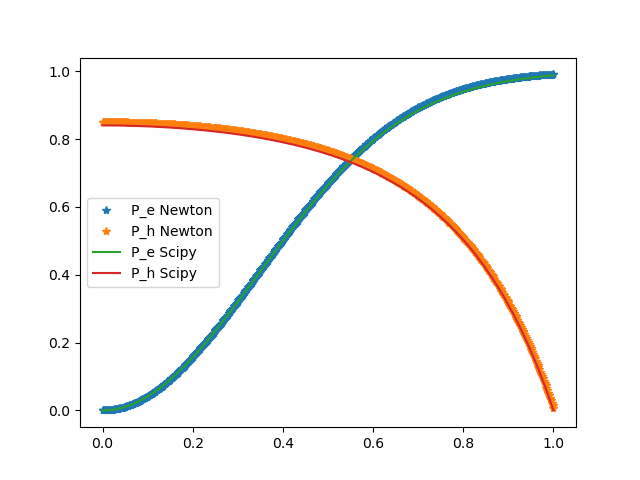
\includegraphics[scale=0.6]{../pictures/NewtonScipyMetod_epoch_512.png}
\end{figure}

\IncMargin{1em}
\begin{algorithm}[h]
	\SetKwData{Left}{left}
	\SetKwData{This}{this}
	\SetKwData{Up}{up}
	\SetKwFunction{Union}{Union}
	\SetKwFunction{FindCompress}{FindCompress}
	\SetKwInOut{Input}{input}\SetKwInOut{Output}{output}
	\Input{The Boundary value Problem}
	\Input{The Mesh $\mathcal{M}$}
	\Input{An initial guess of $Y_{\mathcal{M}}$}
	\Input{A maximal tolerance TOL}
	\Input{A maximal number of iterations}
	\Output{The Solution  $Y_{\mathcal{M}}$}
	\Output{The final residual error }
	\BlankLine
	$\text{RES} \leftarrow  1000$ \;
	$NbIterations \leftarrow 0$\;
	Initialize $w_{\mathcal{M}}$ as a vector of size 2N\;
	\BlankLine
	\While{$RES > TOL$ and NbIterations < MaxNbIterations}{
		\For{i=1 to 2N}{
			Construct $S_i$\;
			Construct $R_i$\;
		 	Construct $q_i =-\textbf{N}_{\mathcal{M}}y_i$\;	}
		Construct $A$\;
		Construct $\beta$\;
		\BlankLine
		Solve $A  w_{\mathcal{M}} = \hat{\beta}$\;
		\BlankLine
		{\For{i=1 to 2N}
			{$y_i \leftarrow y_i + \left( w_{\mathcal{M}}\right)_i $ }}
		\BlankLine
		$RES \leftarrow ||w_{\mathcal{M}}||$\;
		$NbIterations \leftarrow NbIterations + 1$\;
	}
	\If{$RES \leq TOL$}{
		//The method has converged \;
		\Return	Y\;
	}
	\Else{
		//The method has converged \;
		\Return Error : No Convergence
	}
	
	
\caption{Newton's Method Solver for BVP}\label{alg:algo_newton}
\end{algorithm}
\DecMargin{1em}


\subsection{Application to field lines}
The McIntyre model is a fully 1D model where the electron and holes path are assumed to be a straight line, often took from the bottom to the top of the device. In this work we wish to have accurate values of breakdown probability in all the device volume. To this purpose we use electric field streamline to model the carriers transport inside the device. While this modelization might be less accurate than a drift-diffusion model, it would not be consistent with the McIntyre model, where electrons and holes are assumed to follow the same path.
The field lines are computed straightforwardly using simple Euler scheme with adaptive step to ensure a good distribution of points along the line.
\begin{equation}
	\frac{dX(s)}{ds} = \vec{F}_{electric}
\end{equation}
Then the streamline is \[ \{X(s) \text{ for } s \in [s_0, s_f]   \} \]
Our Euler method then reads : 
\begin{align}
	&\frac{X(s+ds)-X(s)}{ds} = \vec{F}_{electric}(X(s)) \\
	\implies & X(s+ds) = X(s) + \underbrace{ds\vec{F}_{electric}(X(s))}_{dX}
\end{align}
So with the discretization, calling $X^k$ the approximation of $X(k*ds)$ we have : 
\begin{align}
&\frac{X^{k+1}-X^k}{ds} = \vec{F}_{electric}(X^k) \\
\implies & X^{k+1} = X^k + \underbrace{ds\vec{F}_{electric}(X^k)}_{dX^k}
\end{align}
This operation is computed both forward (hole motion) and backward (electron motion). We then interpolate the electric field on the line. We set one extremity of the line as it's beginning and the other end as it's end. We can now obtain a function E(x) where x is the distance from the beginning of the line and E(x) is the norm of the electric field at this point. The streamline and this function are represented in figures \ref{fig:electricfieldplot} and \ref{fig:streamline1}.

\begin{figure}[h]
\caption{Field line of electric field inside the device}
\centering
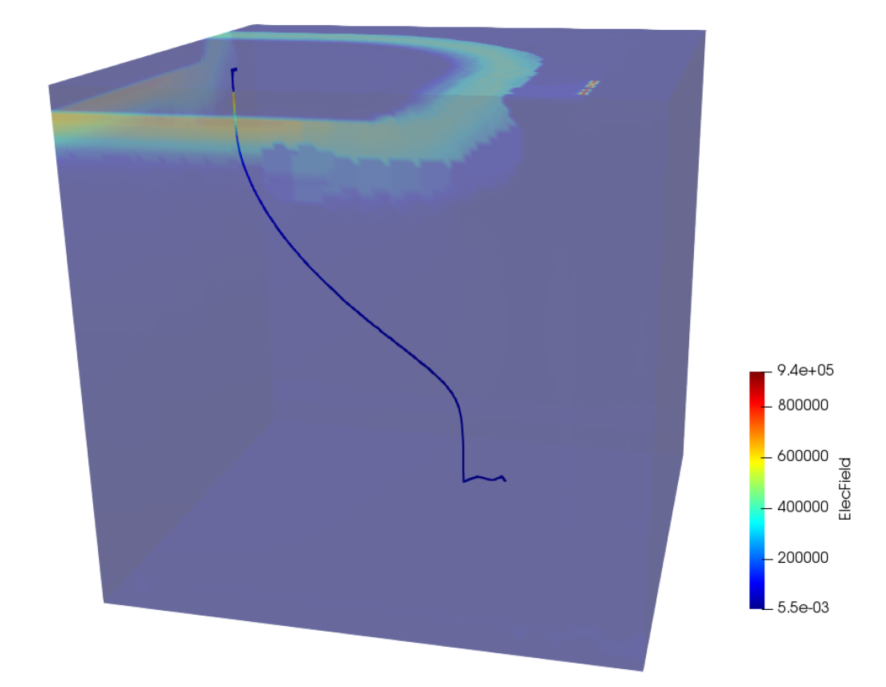
\includegraphics[scale=0.4]{../pictures/SL1.png}
\label{fig:streamline1}
\end{figure}

\begin{figure}[hbtp]
\caption{Plot of the electric field norm along the field line}
\centering
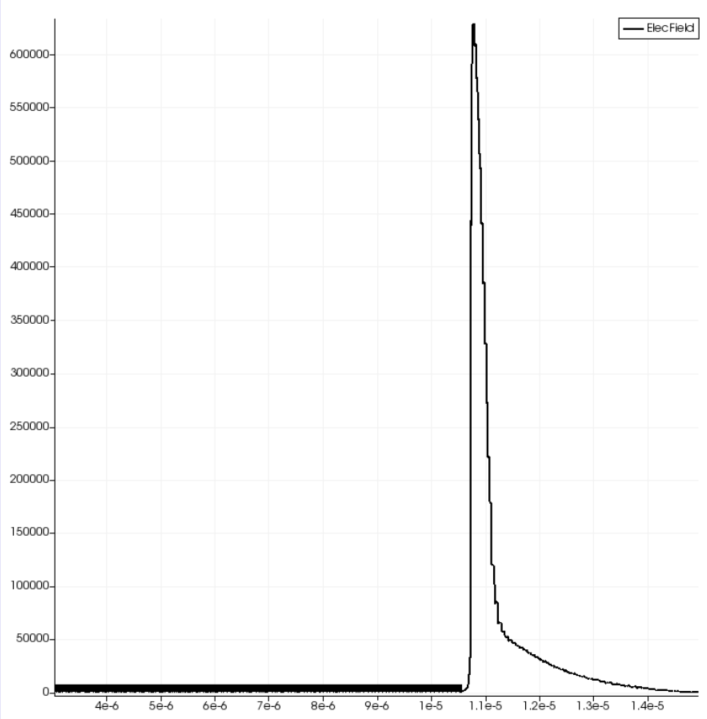
\includegraphics[scale=0.45]{../pictures/ElectricField.png}
\label{fig:electricfieldplot}
\end{figure}

We can now compute the impact ionization coefficients, requirend to compute the McIntyre's model, in this work we choose the local coefficient from Van Overstraeten and De Man \cite{van_overstraeten_measurement_1970}.

We can compute the breakdown probability over multiple streamlines starting from multiple points inside the device and plot them to have an idea of the breakdown probability inside the device, see figure .

\begin{figure}[hbtp]
\caption{Breakdown Probability computed over multiple streamlines}
\centering
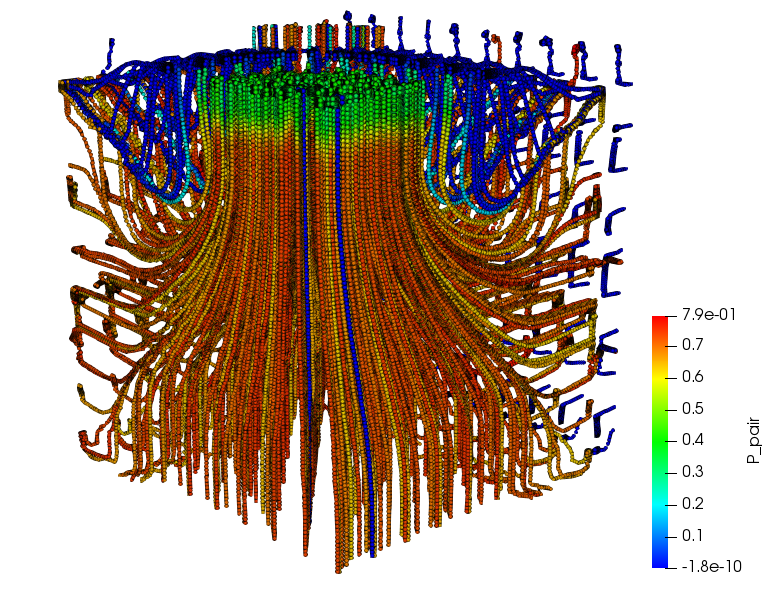
\includegraphics[scale=0.50]{../pictures/MultipleStreamlinesBrP.png}
\end{figure}


\section{Jitter modeling}
\subsection{Drif-Diffusion model}
The jitter in SPAD devices is made of multiple phenomena such as depth of photon absorption, carrier transport timing, avalanche build-up,quench circuit statistics etc. \\In the present work, we focus on the modeling of the carrier transport part. To do so, we \underline{put together} the streamlines and the advection-diffusion equation with variable velocity and diffusion.
Let us consider that a photon absorption at a given point $x_0$ leads to the creation of an electron-hole pair, we want to simulate the timing for the electron to reach the avalanche zone, we assume that this zone is represented by the location of the maximum electric field, denoted $x_{E_{max}}$ . Let $f : (x,t) \mapsto f(x,t)$ the probability distribution of an electron \underline{presence}. We assume that the electron will drift along the electric field streamline. At time $t=0$, f is a Dirac distribution, in order to be able to compute a solution numerically, we start a time $t_0 = \delta t$ where $\delta t$ is as small as possible. We then take the assumption that $D(x) = D(x_0)$ and $u(x) = u_(x_0)$, the analytical solution of the advection-diffusion applies. 

 Hence, f verify the following equation : 
 \[ \forall x \in \left[ x_s, x_{max} \right]  \text{ and } t \in \left[ t_0, T \right] \]
\begin{equation}\label{eq:GeneralAD}
\frac{\partial f}{\partial t}(x,t) = 
	- \frac{\partial( u \cdot f )}{\partial x}(x,t)
	+ \frac{\partial}{\partial x}\left(D \cdot \frac{\partial f }{\partial x}\right)(x,t)
\end{equation}
With the following initial condition : 
\begin{equation}
f(x, t=t_0) = \frac{1}{\sqrt{4 \pi D(x_0) t_0}} exp(-\frac{(x-v(x_0)t_0)^2}{4D(x_0)t_0}
\end{equation}
And setting an absorbing boundary condition at $x_s=x_{E_{max}}$:
\begin{equation}
\frac{\partial f}{\partial t}(x_s,t) = 
	\frac{\partial}{\partial x}\left(D \cdot \frac{\partial( f )}{\partial x}\right)(x_s,t)
\end{equation}
Let $T_e$ the time for the electron to reach the avalanche region. It is straightforward that the probability that $T$ is less than $t$ is:
 \[P_r(t<T) =  F_{Pr}(t) = 1 - \int_{x_0}^{x_{max}} f(x, t) dx \]
From this cumulative distribution function, we can find back the distribution of T:
\begin{equation}
f_T (t) = \frac{F_{Pr}(t)}{dt}
\end{equation}
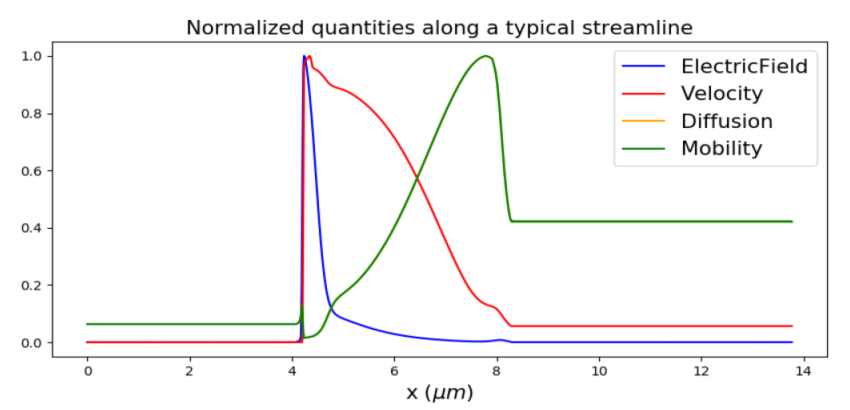
\includegraphics[scale=0.5]{../pictures/PythonVelocityMobilityDiffusionElectricField.png} 

\subsection{Numerical solution}
First, we discretize the streamline $\Omega$ as \[\Omega_h = \left\lbrace x_s = x_0, x_1, x_2, \cdots, x_{N-1}, x_N = x_{max} \right\rbrace \]
And time interval as : 
\[[t_0, t_{max}] = \left\lbrace t_0 = t_0, t_1, t_2, \cdots, t_{M-1}, t_M = t_{max} \right\rbrace \]
The approximation of the solution is noted :
 \[f(x_i, t_k) \simeq f_i^k \: \: \:   \text{    for } i \in \left\lbrace 0, \cdots, N\right\rbrace  \text{ and } k \in \left\lbrace 0, \cdots, M \right\rbrace  \]
The equation is solved by the mean of the finite difference method, more precisely we use a modified Crank-Nicholson method. The differentiation of the equation reads : 
\useshortskip
\begin{align*}\label{eq:CrankNicolson}
\frac{f_i^{k+1} - f_i^{k}}{dt} =& \frac{1}{2} \left[ - u_i \frac{f_{i+1}^{k+1} - f_{i-1}^{k+1}}{2h} 
				+ D_i \frac{f_{i+1}^{k+1} - 2 f_{i}^{k+1} + f_{i-1}^{k+1}}{h^{2}}  \right] \\
				+& \frac{1}{2} \left[-f_i^k \frac{u_{i+1} - u_{i-1} }{2h}
				+ \frac{D_{i+1} - D_{i-1} }{2h} \frac{f_{i+1}^{k+1} - f_{i-1}^{k+1}}{2h} \right] \\ 								
				+ &\frac{1}{2} \left[ - u_i \frac{f_{i+1}^{k} - f_{i-1}^{k}}{2h} 
				+ D_i \frac{f_{i+1}^{k} - 2 f_{i}^{k} + f_{i-1}^{k}}{h^{2}} \right] \\
				+ &\frac{1}{2} \left[-f_i^k \frac{u_{i+1} - u_{i-1} }{2h}
				+ \frac{D_{i+1} - D_{i-1} }{2h} \frac{f_{i+1}^{k} - f_{i-1}^{k}}{2h} \right] \
\end{align*}
It is then straightforward that the resulting scheme will be a linear system to solve with a matrix vector product as right hand side member: 
\[ A F^{k+1} = B F^k\]

The corresponding algorithm would then be :

\IncMargin{1em}
\begin{algorithm}[h]
	\SetKwData{Left}{left}
	\SetKwData{This}{this}
	\SetKwData{Up}{up}
	\SetKwFunction{Union}{Union}
	\SetKwFunction{FindCompress}{FindCompress}
	\SetKwInOut{Input}{input}\SetKwInOut{Output}{output}
	\Input{The initial condition}
	\Input{The space step h and time step dt }
	\Input{The times $t_0$ and $t_{max}$}
	\Output{The Solution  $F^M$}
	\BlankLine
	$\text{time} \leftarrow  t_0$ \;
	Initialize $F$ as a vector of size N with f{initial} values\;
	Construct the matrix A and B defined previously.
	\BlankLine
	\While{$time <= t_{max}$}{
		$Y \leftarrow B F$ \\
		Solve $AX = Y $\\
		$F \leftarrow X$ \\
		$time \leftarrow time + dt$
	}
	\BlankLine
	return F
	
	
\caption{Crank Nicolson algorithm}\label{alg:cn}
\end{algorithm}
\DecMargin{1em}

\section{Results and comparisons with experiments}
\begin{figure}[h]
\caption{Comparison of Breakdown Voltage obtained by McIntyre model versus experiments for multiple SPAD designs}
\centering
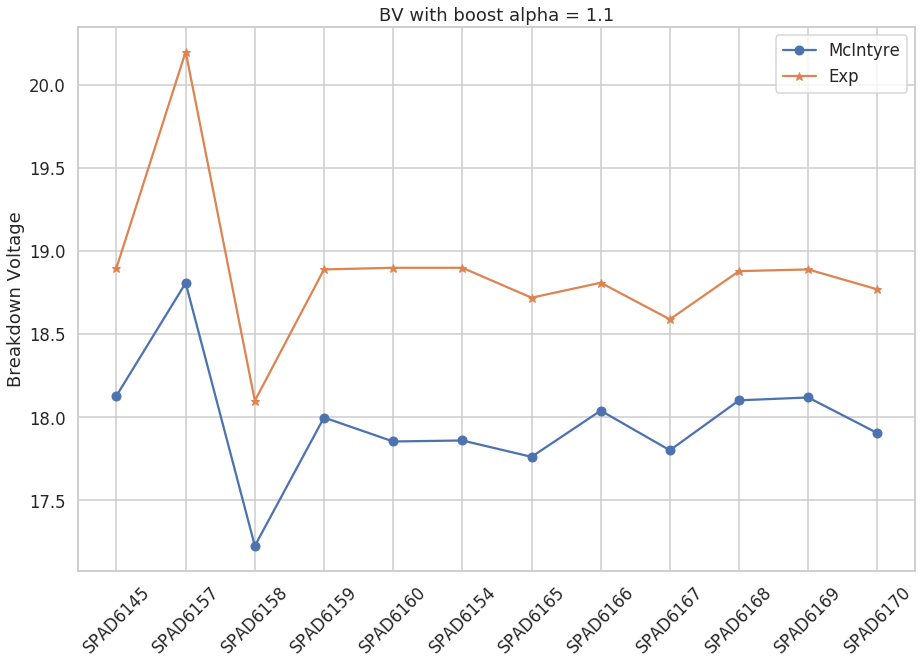
\includegraphics[scale=0.28]{../pictures/BvMcIntyreExp.png}
\end{figure}


\section{Discussion}

\newpage
\newpage
\nocite{*}
\bibliographystyle{apalike}
\bibliography{../biblio/essderc2k21}


















\end{document}